% latex example

\documentclass[10pt]{article}

   \addtolength{\oddsidemargin} {-0.9in}
   \addtolength{\textwidth}{1.7in}
   \addtolength{\topmargin}{-1.2in}
   \addtolength{\textheight}{2in}
   \linespread{1.1}
   \usepackage{graphicx}
   \usepackage{fancyhdr}
   \usepackage{url}
   \usepackage{amsmath,amssymb}
   \usepackage{comment}
   \pagestyle{fancy}
\lhead{} \chead{} \rhead{} \cfoot{} \rfoot{\thepage}
\renewcommand{\headrulewidth}{0.0pt}
\renewcommand{\footrulewidth}{0.4pt}
\usepackage{xcolor}
\definecolor{mygray}{gray}{0.9}
\usepackage[colorlinks=true,linkcolor=blue,citecolor=blue,urlcolor=blue]{hyperref}
\usepackage{chemmacros}

\usepackage{listings}
\usepackage{color} %red, green, blue, yellow, cyan, magenta, black, white
\definecolor{mygreen}{RGB}{28,172,0} % color values Red, Green, Blue
\definecolor{mylilas}{RGB}{170,55,241}

\lstset{language=Matlab,%
    breaklines=true,%
    morekeywords={matlab2tikz},
    keywordstyle=\color{blue},%
    morekeywords=[2]{1}, keywordstyle=[2]{\color{black}},
    identifierstyle=\color{black},%
    stringstyle=\color{mylilas},
    commentstyle=\color{mygreen},%
    showstringspaces=false,%without this there will be a symbol in the places where there is a space
    numbers=left,%
    numberstyle={\tiny \color{black}},% size of the numbers
    numbersep=9pt, % this defines how far the numbers are from the text
    emph=[1]{for,end,break},emphstyle=[1]\color{red}, %some words to emphasise
}

\begin{document}

\begin{center}
{\Large\bf Homework \#10}\\
 {\bf Name: Andrea Livingston}\\
 {\bf Due: December 16th, 2016}\\
 {\bf CBE660: Intermediate Problems in Chemical and Biological
Engineering\; -\; Fall 2016}\\
Department of Chemical and Biological Engineering, University of Wisconsin-Madison
\end{center}

\noindent\colorbox{mygray}{\begin{minipage}{\textwidth}
  {\bf Problem 1}. Solve Exercise 4.33. \\
  Let $X_i = 1, 2, ..., n$ be statistically independent, normally distributed random variables with zero mean and unit variance. Consider the random variable Y to be the sum of squares $Y = X_1^2 + X_2^2 + ... + X_n^2$. \\ \\
  \textit{4.33.a} Find Y's probability density. This density is known as the $\chi^2$ density with $n$ degrees of freedom, and we say $Y \sim \chi_n^2$. Show that the mean of this density is $n$. \\ \\
  \textit{4.33.b} Repeat for the random variable $Z=\sqrt[]{X_1^2 + X_2^2 + ... + X_n^2}$. This density is known as the $\chi$ density with $n$ degrees of freedom. 
  
\end{minipage}}
\\

{\em Solution:}   
\\
\\
{\bf 4.33.a \\ Chi-Squared Distribution}
\\
\\
Begin with the normally distributed variable $X$. The pdf for a normally distributed variable is

\[ f_X(x)=\frac{1}{\sqrt{2\pi}\sigma}exp\left[ \frac{-(x-\sigma)^2}{2\sigma^2} \right] \]
For a mean of zero and the variance of one this becomes

\[ f_X(x)=\frac{1}{\sqrt{2\pi}}exp\left[ \frac{-x^2}{2} \right] \]
\\
If we let $Y=X^2$ then $Y$ also has a chi-squared distribution with one degree of freedom.

\[ f(y) = y=x^2 \]
\[ f^{-1}(y)=x=\sqrt(y) \]
\\

\noindent
Using the change of variables equation (equation 4.23)
\[ f_Y(y)=f_X(f^{-1}(y)) \left| det\frac{df^{-1}(y)}{dy} \right| \]
\[ \left| det\frac{df^{-1}(y)}{dy} \right| = \frac{d}{dy}y^{1/2} = \frac{1}{2 \sqrt{y}} \]
\[  f_Y(y)= f_X(\sqrt{y})\frac{1}{2 \sqrt{y}} \]
\\

\noindent
But because $\pm x$ gives the same results
\[ f_Y(y)= f_X(\sqrt{y})\frac{1}{2 \sqrt{y}} + f_X(-\sqrt{y})\frac{1}{2 \sqrt{y}}\]

\[ f_X(\sqrt{y})=f_X(-\sqrt{y}) = \frac{1}{\sqrt{2\pi}}exp\left[ \frac{-y}{2} \right] \]
\[ f_Y(y)=\frac{1}{\sqrt{2\pi}}exp\left[ \frac{-y}{2} \right]\frac{1}{2\sqrt{y}} + \frac{1}{\sqrt{2\pi}}exp\left[ \frac{-y}{2} \right] \frac{1}{2\sqrt{y}} \]
\[ f_Y(y)=\frac{1}{\sqrt{2\pi y}}exp\left[\frac{-y}{2}\right] \]
\\
\\
Given the characteristic function for $X$, the characteristic function of a one-dimensional $Y$ can be found 

\[ \varphi_X(t)=E \left[ e^{itx} \right] = \int_{-\infty}^{\infty}e^{itx}f_X(x)dx \]
\[ \varphi_Y(t)=\int_{-\infty}^{\infty}e^{i t y}f_Y(y)dy\]
\[ \varphi_Y(t)=\int_{-\infty}^{\infty}e^{i t y} \frac{1}{\sqrt{2\pi y}}exp\left[\frac{-y}{2}\right] dy \]
\[ \varphi_Y(t)= \frac{1}{\sqrt{2\pi}}  \int_{-\infty}^{\infty}e^{i t y} \frac{1}{\sqrt{y}}  exp\left[\frac{-y}{2}\right] dy\]
\[ \varphi_Y(t)= \frac{1}{\sqrt{1-2it}} \]
\\
Now expanding this to an n-dimensional case using the property for $\eta=\epsilon_1+\epsilon_2+ \dots \epsilon_n$ (equation 4.8)

\[\varphi_{\eta}(t)=\varphi_{\epsilon_1}(t)\varphi_{\epsilon_2}(t) \dots \varphi_{\epsilon_n}(t) \]
\\
and defining $Y=\Sigma_{i=1}^n X_i^2$ the characteristic equation becomes

\[ \varphi_Y(j \omega)=\frac{1}{(1-2it)^{\frac{n}{2}}} \]
Moving from the characteristic function back to the probability density (equation on p.354)

\[ f_Y(y)= \frac{1}{2\pi}\int_{-\infty}^{\infty}e^{-ity}\varphi_Y(t)dt \]
\[ f_Y(y)= \frac{1}{2\pi}\int_{-\infty}^{\infty}e^{-ity} \frac{1}{(1-2it)^{\frac{n}{2}}} dt \]
Defining the gamma function

\[ \Gamma(z)=\int_0^{\infty}x^{z-1}e^{-x}dx \]
\[ \Gamma(\frac{n}{2})= \int_0^{\infty}y^{\frac{n}{2}-1}e^{-\frac{n}{2}}dy \]
Taking the inverse transform of the characteristic function gives the n-dimensional $\chi ^2$ probability density for $y\geq 0$. For $y < 0$ then $f_Y(y)=0$

\[ f_Y(y)=\frac{1}{2^{n/2}\Gamma(n/2)}y^{n/2-1}e^{-y/2} \]
\\
\\


\noindent
{\bf 4.33.b   \\  CHI DISTRIBUTION}
\\
\\

\noindent
For the chi distribution, we now consider 
$ Z=\sqrt{ \sum_{i=1}^{n} (\frac{X_i-\mu_i}{\sigma_i})^2 }=\sqrt{x} $. Beginning with the  $\chi ^2$ probability density

\[ f_Y(y)=\frac{1}{2^{n/2}\Gamma(n/2)}y^{n/2-1}e^{-y/2} \]
Apply the change of variables formula with the mapping relationship $z=y^2$ and $y=\sqrt{z}$.

\[ g(z)=f(y)\frac{dy}{dz}=f(z^2)2z \]
\[ g(z)=f_Z(z)=\frac{2z}{2^{n/2}\Gamma(n/2)}(z^2)^{n/2-1}e^{-z^2/2} \]
\[ f_Z(z)=\frac{2 z^1z^{n-2}e^{-z^2/2}}{2^{n/2}\Gamma(n/2)} \]
Simplifying $z^1z^{n-2}=z^{n-1}$ and $\frac{2}{2^{n/2}}=n^{1-n/2}$ gives the Chi probability density 
\[ f_Z(z)=\frac{2^{1-n/2} z^{n-1}e^{-z^2/2}}{\Gamma(n/2)} \]






\newpage

\noindent\colorbox{mygray}{\begin{minipage}{\textwidth}
  {\bf Problem 2}. Solve Exercise 4.31. \\ \\
  A common model for the temperature dependence of the reaction rate is the Arrhenius model. In this model the reaction rate (rate constant, k) is given by 
\[k = k_0exp(-E/T)\]
in which the parameter $k_0$ is the preexponential factor, $E$ is the activation energy scaled by the gas constant, and $T$ is the temperature in Kelvin. We wish to estimate $k_0$ and $E$ from the measurements of the reaction rate at different temperatures. In order to use linear least squares, we take the logarithm of the reaction rate 
\[ln(k) = ln(k_0) - E/T\]
Assume you have made measurements of the rate constant at 10 temperatures evenly distributed between 300 and 500K. Model the measurement process as the true value plus measurement error, $e$, which is distributed normally with zero mean and 0.001 variance. Choose the true value of the parameters to be $ln(k_0) = 1$, $E=100$. \\ \\
  \textit{4.31.a} Generate a set of experimental data for this problem. Estimate the parameters from these data using least squares. Plot the data and the model fit using both (T,k) and (1/T, ln k) as the (x,y) axes. \\ \\
  \textit{4.31.b} Calculate the 95\% confidence intervals for your parameter estimates. What are the coordinates of the semi-major axes of the ellipse corresponding to the 95\% confidence interval? \\ \\
  \textit{4.31.c} What are the coordinates of the corners of the box corresponding to the 95\% confidence interval? \\ \\
  \textit{4.31.d} Plot your results by showing the parameter estimate, ellipse and box. Are the parameter estimates highly correlated? Why or why not? 
  
  \end{minipage}}
\\

{\em Solution:}   
\\
{\bf 4.31.1}\\
Experimental data was generated according to 
\[ ln(k)=lnk_0-E/T+e \]
\[ ln(k)=1-100/T+e \]
\\
Using the least squares regression, the parameters for $k_0$ and $E$ were fitted.The fitted results were plotted against the 'experimental' data.
\[ x_{ls}=(A^TA)^{-1}A^T b\]

{\bf 4.31.b} \\
The 95$\%$ confidence interval was determined using $\chi^2(n_p=2,0.95)$. 
Solving this equation
\[ (x-m)^TP^{-1}(x-m) \leq \chi^2(n_p,\alpha) \]
leads to 
\[ |{\hat \theta}-\theta_0|_i \leq \left( \chi^2(n_p,\alpha)\sigma^2(X^TX)_{ii}^{-1}  \right)^{1/2} \]
and
\[ c_i=(\chi^2(n_p,\alpha)\sigma^2(A^TA)^{-1}_{ii})^{1/2} \]
\\
The resultant confidence intervals were
\[ ln(k)=1.000 \pm 0.1508\]
\[ E=100.1211 \pm 57.15\]
\\
\\
{\bf 4.31.c} \\
The corresponding corners of the bounding box are given by\\
\[1.148791 \;\; 1.58080e+02\] \\
\[1.024507 \;\; 1.00121e+02\] \\
\\
{\bf 4.31.d} 
\\
Yes, the system is highly coordinated.Changing one variable would change the covariance matrix which would have a significant impact on the other. 

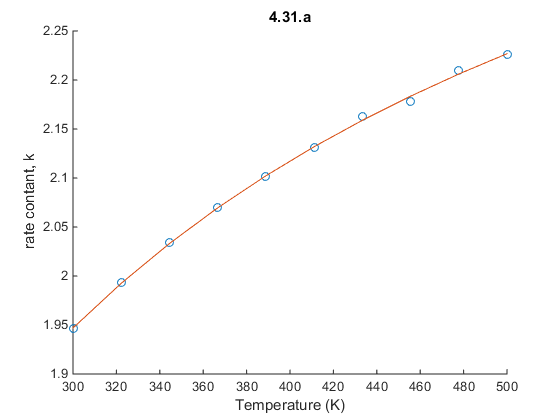
\includegraphics{CBE660_Assign10__2a.png} \\
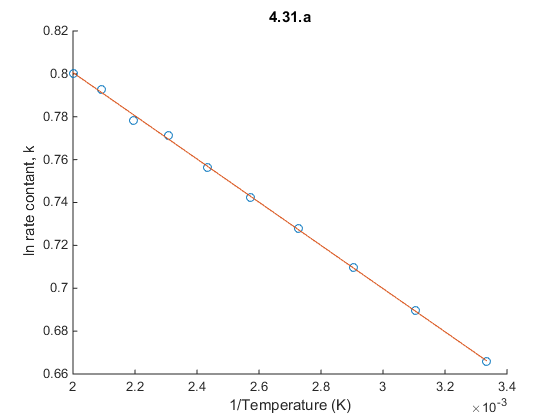
\includegraphics{CBE660_Assign10__2b.png} \\
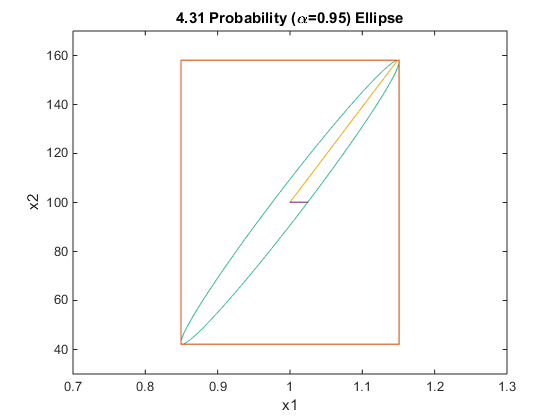
\includegraphics{CBE660_Assign10__2c.png}

\lstinputlisting{CBE660_Assign10.m}

\newpage

\noindent\colorbox{mygray}{\begin{minipage}{\textwidth}
  {\bf Problem 3}.  Solve Exercise 4.22. \\ \\
  Given the normally distributed random variable $\xi\in{\mathbb R}^n$, consider the random variable, $\eta \in {\mathbb R}^n$, obtained by the linear transformation
\[ \eta = A\xi \]
in which $A$ is a nonsingular matrix. Using the result on transforming probability densities show that if $\xi \sim N(m,P)$, then $\eta \sim N(Am, APA^T)$. This result establishes that invertible linear transformations of nonsingular normal random variables are normal. 
\end{minipage}}
\\

{\em Solution:}  
\\
\\
Considering the random variable $\eta$ transformed as
\[ \eta=A \xi \]
Given that this is a linear transformation, we can say
\[ \eta=f(\xi) \]
\[ \xi=f^{-1}(\eta) \]
\[ \eta=A \xi \]
\[ \xi=A^{-1}\eta \]
\\

\noindent
Because the variable associated with $\eta$ is $y$ and the variable associated with $\xi$ is $x$
\[ x=A^{-1}y \]
\\

\noindent
From equation 4.23
\[ p_\eta(y)=p_\xi(f^{-1}(y))\left|det \frac{dA^{-1}\eta}{d \eta} \right| \]

\noindent
Taking the derivative with respect to $\eta$ 
\[ p_\eta(y)=p_\xi(f^{-1}(y))\left|det \; A^{-1}\right| \]

\noindent
Simplifying the determinant term using properties of linear algebra
\[ det(A^{-1})=\frac{1}{det(A)} \]
\[ p_\eta(y)=p_\xi(f^{-1}(y))\frac{1}{det\; A}\]
\\

\noindent
By inspection $|x|=\sqrt{x\;x}$. Extending this concept to the determinants, which are scalars
\[ p_\eta(y)=p_\xi(f^{-1}(y))\sqrt{\frac{1}{det\; A} \frac{1}{det\; A} } \]
\\

\noindent
From equation 4.12 for the probability density of $\xi \sim N(m,P)$ where $m$ is the mean and $P$ is a real, symmetric positive definite matrix (covariance matrix of $\xi$)
\[ p_{\xi}(x)=\frac{1}{(2\pi)^{n/2}(det\;P)^{1/2}}exp\left[ \frac{-1}{2}(x-m)^TP^{-1}(x-m) \right] \]
\[  p_{\xi}(f^{-1}(y)) = p_{\xi}(A^{-1}y) =\frac{1}{(2\pi)^{n/2}(det\;P)^{1/2}}exp\left[ \frac{-1}{2}(A^{-1}y-m)^TP^{-1}(A^{-1}y-m) \right] \]
\\

\noindent
Substituting $p_{\xi}(f^{-1}(y))$ into the expression for $p_\eta(y)$

\[ p_\eta(y)=\sqrt{\frac{1}{det\;A} \frac{1}{det\;A} } \;\; \frac{1}{(2\pi)^{n/2}(det\;P)^{1/2}}exp\left[ \frac{-1}{2}(A^{-1}y-m)^TP^{-1}(A^{-1}y-m) \right]   \]
\[ p_\eta(y)=\sqrt{\frac{1}{det\;A} \frac{1}{det\;A} \frac{1}{(2\pi)^n (det\;P)} } exp\left[ \frac{-1}{2}(A^{-1}y-m)^TP^{-1}(A^{-1}y-m) \right]  \]
\\

\noindent
Introducing the identity matrix $I=A^{-1}A$ and rearranging

\[ p_\eta(y)=\sqrt{\frac{1}{det\;A} \frac{1}{det\;A} \frac{1}{(2\pi)^n (det\;P)} } exp\left[ \frac{-1}{2}(I(A^{-1}y-m))^TP^{-1}(I(A^{-1}y-m)) \right]  \]

\[ p_\eta(y)=\sqrt{\frac{1}{det\;A} \frac{1}{det\;A} \frac{1}{(2\pi)^n (det\;P)} } exp\left[ \frac{-1}{2}(A^{-1}A(A^{-1}y-m))^TP^{-1}(A^{-1}A(A^{-1}y-m)) \right]  \]

\[ p_\eta(y)=\sqrt{\frac{1}{det\;A} \frac{1}{det\;A} \frac{1}{(2\pi)^n (det\;P)} } exp\left[ \frac{-1}{2}(A^{-1}(AA^{-1}y-Am))^TP^{-1}(A^{-1}(AA^{-1}y-Am)) \right]  \]

\[ p_\eta(y)=\sqrt{\frac{1}{det\;A} \frac{1}{det\;A} \frac{1}{(2\pi)^n (det\;P)} } exp\left[ \frac{-1}{2}(A^{-1}(y-Am))^TP^{-1}(A^{-1}(y-Am)) \right]  \]

\[ p_\eta(y)=\sqrt{\frac{1}{det\;A \;(det\;P) \; det\;A } } \frac{1}{(2\pi)^{n/2} }exp\left[ \frac{-1}{2}(y-Am)^T A^{-1T} P^{-1}A^{-1}(y-Am) \right]  \]
\\

\noindent
Now let $det(A)=det(A^T)$ and $A^{-1T} P^{-1}A^{-1}=(APA^T)^{-1}$

\[ p_\eta(y)=\frac{1}{(2\pi)^{n/2}det\;( APA^T)^{1/2}} exp\left[ \frac{-1}{2}(y-{\bf Am})^T ({\bf APA^T} )^{-1}  (y-{\bf Am}) \right]  \]
\\


\noindent
Comparing this equation to equation 4.12 for $p_{\xi}(x)$ for which $\xi \sim N(m,P)$ 

\[ p_{\xi}(x)=\frac{1}{(2\pi)^{n/2}(det\;P)^{1/2}}exp\left[ \frac{-1}{2}(x-\textbf{m})^T \textbf{P}^{-1} (x-\textbf{m}) \right] \]
\\

\noindent
we can draw parallels to see that $\eta \sim N(Am,APA^T)$


\end{document}


